\chapter*{Вероятность}
\addcontentsline{toc}{chapter}{Вероятность}

\setlength{\epigraphwidth}{.85\textwidth}
\epigraph{Человеческий мозг был создан эволюцией для решения задач, связанных с добычей пропитания в составе небольших кочевых племён в Африканской саванне...
Осуждать наш разум за слабость к азартным играм это всё равно, что жаловаться на то, что наше запястье плохо устроено, потому что мы не можем вытащить руку из наручников.}{---Стивен Пинкер «Как работает мозг»%(Steven Pinker « How the Mind Works»)
}

Мы сталкиваемся с теорией вероятностей каждый день.
Она является основой для изучения статистики, играющую в современном обществе огромную роль при принятии решений.
Но исторически, теория вероятностей берёт своё начало в азартных играх и \emph{умозрительных} экспериментах как те, что будут рассмотрены ниже.

\medskip

Вероятностные задачи могут быть катастрофически контринтуитивными.
Рассмотрим следующий разумно выглядящий вопрос:

\subsection*{Русская рулетка} %( GROUP RUSSIAN ROULETTE)
\rindex{Русская рулетка}

В комнате находятся $n$ вооружённых и сердитых людей.
При каждом ударе часов, все одновременно поворачиваются кругом и стреляют в случайного человека.
Те, в кого попали, умирают, выжившие крутятся и снова стреляют со следующим ударом часов.
В конце концов, либо все умирают, либо остаётся один выживший.

Если $n$ растёт, какова предельная вероятность того, что кто-то останется жив?

\paragraph{Решение:} Удивительным образом, вероятность вовсе и не стремится к пределу.
При возрастании $n$ вероятность меняется слегка, но беспрестанно, в зависимости от дробной части натурального логарифма $n$.%
\footnote{Этот результат описан в статье 
T. van de Brug, W. Kager, R. Meester, ``The asymptotics of group Russian roulette''.
\emph{Markov Process. Related Fields} 23 (2017), 35--66.}

\medskip

Следующая задача тесно связана со знаменитым «парадоксом Монти Холла» (смотри ниже), который лет десять назад породил бурю смятений и споров.

\subsection*{Обратная сторона монеты}% ( THE OTHER SIDE OF THE COIN)
\rindex{Обратная сторона монеты}

Монета, у которой обе стороны --- решки, монета, у которой обе стороны --- орлы, и обычная монета, кладутся в мешок.
Случайным образом выбираем одну монету и подбрасываем.
Выпадает решка.
Какова вероятность того, что другая сторона монеты тоже решка?

\paragraph{Решение:}
Очевидно, что выбранная монета либо обычная, либо двурешечная, таким образом, у её другой стороны одинаковые шансы оказаться орлом или решкой.
Так?
Нет, неверно.

Можно думать об этом следующим образом: если монета была обычная, то \emph{мог бы} выпасть орёл, тогда как у двурешечной выбора нет, поэтому предполагается, что скорее всего монета двурешечная.

Это известно игрокам в Бридж (а сто лет назад игрокам в Вист) как «принцип ограниченного выбора».

Проще говоря, представим, что монета подбрасывается десять раз, и каждый раз выпадает орёл.
Она всё ещё \emph{может быть} обычной монетой, но скорее всего эта монета двуорловая.
То же самое верно и после первого броска.

Один из способов подсчитать вероятность напрямую таков:
обозначим все шесть \emph{сторон} наших монет ---
на двурешечной монете обозначим стороны Р1 и Р2, на двуорловой --- О1 и О2, а на обычной --- Р3 и О3.
Когда мы выбираем и подкидываем монету, шанс выпасть у каждой из шести сторон одинаковый.
Из трёх решек, у Р1 и Р2 на другой стороне решка, таким образом, искомая вероятность $2/3$.\heart

Источник: Кто знает, я использовал эту задачу, когда преподавал курс элементарной теории вероятностей в университетах Стэндфорта и Эмори.

\medskip

Парадокс Монти Холла основан на телеигре «Let’s Make a Deal», в которой участников игры (некоторых) просили выбрать одну из трёх дверей в поисках ценного приза.
Ведущий Монти Холл, который знал, где находился приз, открывал вместо выбранной другую дверь: приза за ней не было.
Участникам предоставлялась возможность либо остаться с первоначальным выбором, либо поменяться на третью дверь.
В детстве я смотрел иногда это шоу, и помню, как, примерно половина зрителей кричала участнице: «ОСТАВЛЯЙ!», а другая половина: «МЕНЯЙ!».

Конечно, дверь следует менять.
Если бы эта игра игралась 300 раз, то правильная дверь была бы выбрана \emph{с первого раза} примерно 100 раз.
Остальные 200 игр выиграл бы участник, который бы менял дверь каждый раз!

\medskip

Не отчаивайтесь, если для вас это было очевидно.
Оставшиеся задачи вполне могут поколебать уверенность в вашей вероятностной интуиции.

\subsection*{Потерянный посадочный талон}% (THE LOST BOARDING PASS)
\rindex{Потерянный посадочный талон}

Сто человек выстроились в очередь на посадку в самолёт, но первый в очереди пассажир потерял посадочный талон и садится на случайное место.
Каждый следующий пассажир занимает место согласно своему посадочному талону, если оно свободно, либо, в противном случае, случайно выбирает любое незанятое место.

\medskip

Какова вероятность того, что последний пассажир найдёт своё место незанятым?

\subsection*{Все грани кубика}% (ROLLING ALL THE NUMBERS)
\rindex{Все грани кубика}

В среднем, сколько раз надо бросить кубик до того, как выпадет каждая из шести цифр?

\subsection*{Нечётная череда решек}% (ODD STREAK OF HEADS)
\rindex{Нечётная череда решек}

Сколько раз, в среднем, надо подбросить монету (обычную) до того, как решка выпадет подряд нечётное число раз, а затем орёл? 

\subsection*{Три кубика}% (THREE DICE)
\rindex{Три кубика}

У вас есть возможность поставить 1 доллар на число между 1 и 6.
Далее бросаются три кубика.
Если ваше число не выбрасывается, то вы проиграли доллар.
Если ваше число выпало на одном кубике, то выиграли 1 доллар, если на двух кубиках --- 2 доллара, на трёх --- 3 доллара.

\medskip

Является ли эта ставка выигрышной, нейтральной или проигрышной? Есть ли способ определить это, не делая никаких вычислений?

\subsection*{Намагниченные доллары}% (MAGNETIC DOLLARS)
\rindex{Намагниченные доллары}

Один миллион намагниченных «сюзанн» (монета США номиналом в 1 доллар с изображением Сюзенн Энтони) бросаются в две урны следующим способом: изначально в каждой урне лежит по одной монете, затем все остальные монеты, одна за одной, подкидываются в воздух.
Если в первой урне $x$ монет, а во второй --- $y$, то за счёт магнетизма каждая последующая монета попадает в первую урну с вероятностью $x/(x+y)$, и во вторую с вероятностью $y/(x+y)$.

Сколько вы готовы заплатить вперёд за содержимое урны, в которой в итоге окажется меньше монет?

\subsection*{Торговля вслепую}% (BIDDING IN THE DARK)
\rindex{Торговля вслепую}

Есть возможность купить некий приборчик, стоимость которого для его владельца, насколько вам известно, равномерно распределена между 0 и 100 долларами.
Вы также знаете, что вы можете использовать этот приборчик намного лучше, чем его владелец; так что вы оцениваете его стоимость на $80\%$ больше цены хозяина.

\medskip

Если вы предложите сумму за приборчик больше той, во что его ценит владелец, то он вам его продаст.
Но можно сделать только одно предложение.
Сколько следует предложить?

\subsection*{Случайные интервалы}% (RANDOM INTERVALS)
\rindex{Случайные интервалы}

Точки $1, 2,\dots, 1000$ на числовой прямой разбиты случайным образом на пары и образуют 500 интервалов.
Какова вероятность того, что среди этих интервалов найдётся такой, который пересекает все остальные?

\begin{figure}[h!]
\centering
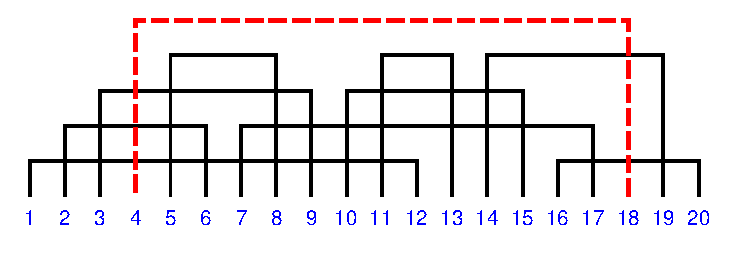
\includegraphics[scale=0.8]{Figs/Probability/ints}
\end{figure}
